%!TEX program = lualatex
\documentclass[11pt]{article}
\usepackage[a4paper, margin=1in, includehead]{geometry}
\geometry{a4paper} 
\usepackage[table, svgnames, dvipsnames]{xcolor}
\usepackage{makecell, cellspace, caption}
\usepackage[utf8]{inputenc}
\usepackage{textcomp}
\usepackage[most]{tcolorbox}
\usepackage{enumitem}
\usepackage{multicol}
\usepackage{graphicx} 
\usepackage{titling}
\usepackage{fancyhdr}
\usepackage{tabularray}
\pagestyle{fancy}
\fancyhf{}
\fancyhfoffset[L]{1cm} % left extra length
\fancyhfoffset[R]{1cm} % right extra length
\rhead{\textbf{\textit{Page-\thepage}}}
\lhead{\textbf{\textit{Test Document for PedalPal}}}
\cfoot{}
\usepackage{amsmath,amssymb}  
\usepackage{bm}  
\usepackage[pdftex,bookmarks,colorlinks,breaklinks]{hyperref}  
\hypersetup{linkcolor=black,citecolor=black,filecolor=black,urlcolor=blue} % black links, for printed output
\usepackage{memhfixc} 
\usepackage{pdfsync}  
\usepackage{fancyhdr}
\usepackage{lmodern}
\usepackage{wrapfig}
\usepackage[page,toc,titletoc,title]{appendix}

\usepackage{fontspec}
\setmainfont{Arial}

\pagestyle{fancy}

\usepackage{titlesec}
\begin{document}
\begin{titlingpage}
\begin{flushright}
    \rule{16cm}{5pt}\vskip1cm
    \textbf{{\fontsize{30}{36}\selectfont Test Document}\\ \vspace{1cm}\huge{for}\\\vspace{1cm}\Huge{PedalPal}\\ \vspace{1.5cm}\LARGE{Version 1.0}\\\vspace{1cm}\LARGE{Prepared by}}
\end{flushright}
\vspace{1.0cm}
\large{\begin{tabular*}{\columnwidth}{@{\extracolsep{\stretch{1}}}*{3}{c}@{}}
    \Large{\textbf{Group \# 4}} & & \Large{\textbf{Group Name: Bit Brewers}} \\
    \\
    \textbf{Raghav Manglik} & \textbf{220854} & \href{mailto:raghavkmanglik@gmail.com}{raghavkmanglik@gmail.com} \\
    \textbf{Amogh Bhagwat} & \textbf{220288} & \href{mailto:amogh.2004b@gmail.com}{amogh.2004b@gmail.com} \\
    \textbf{Srishti Chandra} & \textbf{221088} & \href{mailto:chandra.srishti2403@gmail.com}{chandra.srishti2403@gmail.com} \\
    \textbf{Wadkar Srujan Nitin} & \textbf{221212} & \href{mailto:srujanwadkar@gmail.com}{srujanwadkar@gmail.com} \\
    \textbf{Anaswar K B} & \textbf{220138} & \href{mailto:anaswarkb013@gmail.com}{anaswarkb013@gmail.com} \\
    \textbf{Khushi Gupta} & \textbf{220531} & \href{mailto:khushi07g@gmail.com}{khushi07g@gmail.com} \\
    \textbf{Ananya Singh Baghel} & \textbf{220136} & \href{mailto:ananyabaghel2004@gmail.com}{ananyabaghel2004@gmail.com} \\
    \textbf{Pathe Nevish Ashok} & \textbf{220757} & \href{mailto:nevu.pathe1234@gmail.com}{nevu.pathe1234@gmail.com} \\
    \textbf{Debraj Karmakar} & \textbf{220329} & \href{mailto:debraj2003jsr@gmail.com}{debraj2003jsr@gmail.com} \\
    \textbf{Kaneez Fatima} & \textbf{220496} & \href{mailto:kaneezfatimamehdi7@gmail.com}{kaneezfatimamehdi7@gmail.com} \\
    
\end{tabular*}}

\vspace{1.5cm}
\begin{center}
\large{
\begin{tabular}{l l}
    \textbf{Course:} & \textbf{CS253} \\
    \textbf{Mentor TA:} & \textbf{Mr. Bharat} \\
    \textbf{Instructor:} & \textbf{Prof. Indranil Saha} \\
    \textbf{Date:} & \textbf{January 25, 2024}
\end{tabular}
}
\end{center}
\end{titlingpage}

\titleformat{name=\section}[block]
  {\sffamily\LARGE}
  {}
  {0pt}
  {\colorsectionx}
\titlespacing*{\section}{0pt}{\baselineskip}{\baselineskip}
\newcommand{\colorsectionx}[1]{\colorbox{gray!120}{\parbox{\dimexpr\textwidth-2\fboxsep}{\color{white} \centering \huge{\textbf{Contents}}}}}

\tableofcontents

\newpage
\titleformat{name=\section}[block]
  {\sffamily\LARGE}
  {}
  {0pt}
  {\colorsection}
\titlespacing*{\section}{0pt}{\baselineskip}{\baselineskip}

\newcommand{\colorsection}[1]{\colorbox{gray!120}{\parbox{\dimexpr\textwidth-2\fboxsep}{\color{white}\huge{\textbf\thesection. }\ #1}}}

\section{\centering{\textbf{Revisions}}}
\begin{center}
\begin{tabular}{|c|c|c|c|}
    \hline
    \rowcolor{Gainsboro!60}
    \textbf{Version} & \textbf{Primary Author(s)} & \textbf{Description of Version} & \textbf{Date Completed} \\
    \hline
    \makecell{v1.0} & \makecell{Raghav Manglik \\ Amogh Bhagwat \\ Srishti Chandra \\ Wadkar Srujan Nitin \\ Pathe Nevish Ashok \\ Debraj Karmakar \\ Khushi Gupta \\ Ananya Baghel \\ Anaswar K B \\ Kaneez Fatima \\} & \makecell{First version of the \\ Test Document} & \makecell{29/03/24} \\
    \hline
\end{tabular}
\end{center}

\newpage
\section{\centering{\textbf{Introduction}}}

\newpage
\section{\centering{\textbf{Unit Testing}}}
\subsection{Authentication}
\subsubsection{Registering a User}
\textbf{API Endpoint: } \texttt{/auth/register/} \\
\textbf{Test Owner: } Amogh Bhagwat \\
\textbf{Date: } 25/03/2024 \\
\textbf{Test Description: } This test case is used to check if a user can register successfully. \\
\textbf{Test Results: } User is able to register successfully. If a user with the email already exists, appropriate error message is shown. Authentication token is also generated correctly. \\
\begin{center}
    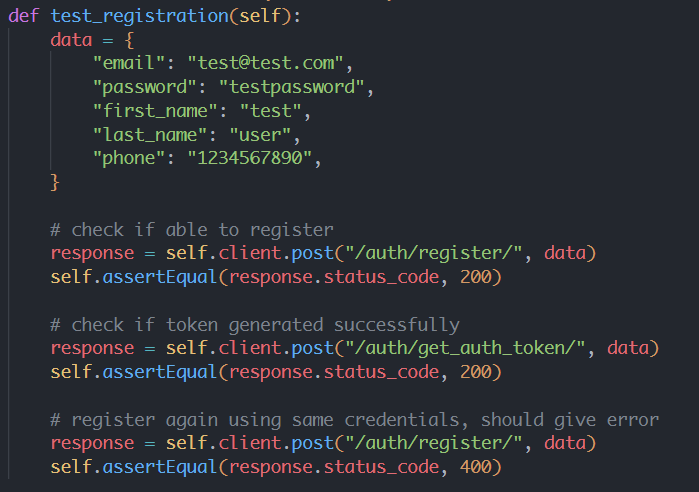
\includegraphics[scale=0.8]{unit_testing_codes/register.png}
\end{center}

\subsubsection{Logging in a User}
\textbf{API Endpoint: } \texttt{/auth/login/} \\
\textbf{Test Owner: } Amogh Bhagwat \\
\textbf{Date: } 25/03/2024 \\
\textbf{Test Description: } This test case is used to check if a user can login successfully. \\
\textbf{Test Results: } User is able to login successfully. If the user enters wrong password or the user does not exist, appropriate error message is shown. \\

\begin{center}
    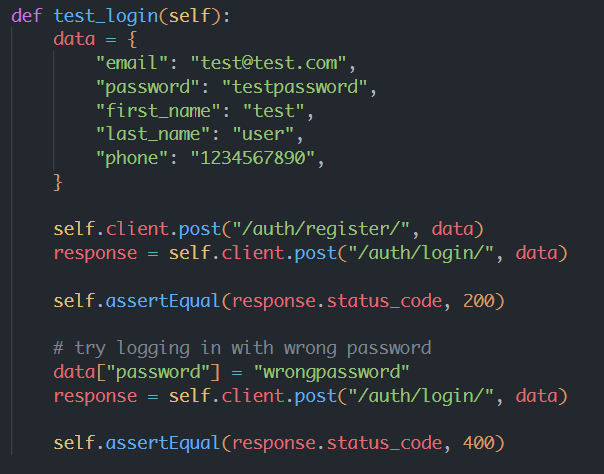
\includegraphics[scale=0.7]{unit_testing_codes/login.png}
\end{center}

\subsubsection{Email Verification}
\textbf{API Endpoint: } \texttt{/auth/verify/} \\
\textbf{Test Owner: } Amogh Bhagwat \\
\textbf{Date: } 25/03/2024 \\
\textbf{Test Description: } This test case is used to check if a user can verify their email successfully. \\
\textbf{Test Results: } User receives the mail containing the link to verify their email successfully. On clicking the link, their email is verified. If the OTP in the link is modified, the verification fails. \\

\begin{center}
    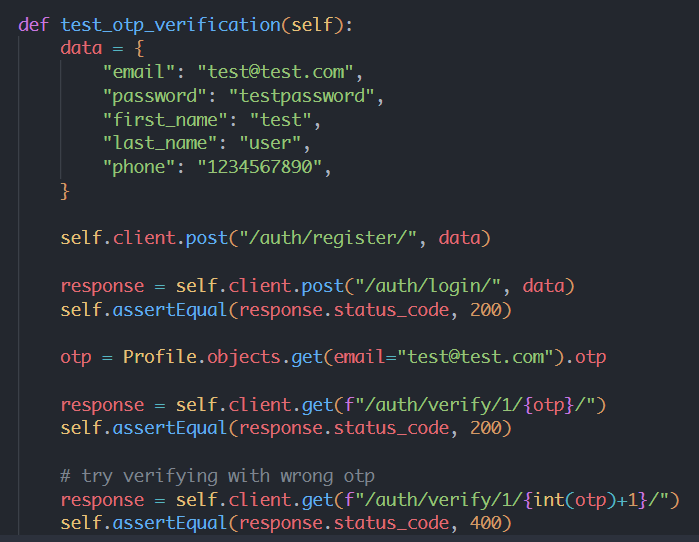
\includegraphics[scale=0.6]{unit_testing_codes/verify.png}
\end{center}

\subsection{Cycle Bookings}
\subsubsection{Starting Ride Instantly}
\textbf{API Endpoint: } \texttt{/booking/book/} \\
\textbf{Test Owner: } Khushi Gupta \\
\textbf{Date: } 26/03/2024 \\
\textbf{Test Description: } This test case is used to check if a user can start a ride instantly by scanning the QR code on the lock. \\
\textbf{Test Results: } User is able to start the ride instantly by scanning the QR code on the lock. The following edge cases were tested - 
\begin{itemize}
    \itemsep 0em
    \item If the user has negative balance in their wallet, they are denied to start the ride.
    \item If the QR code is invalid, appropriate error message is shown.
    \item If the lock has no cycle attached to it, appropriate message is shown.
    \item If the user already has an active ride in progress, they are denied to start another ride.
    \item If the cycle is already booked by some other user, appropriate message is shown.
\end{itemize}
The test database is initialized as follows
\begin{center}
    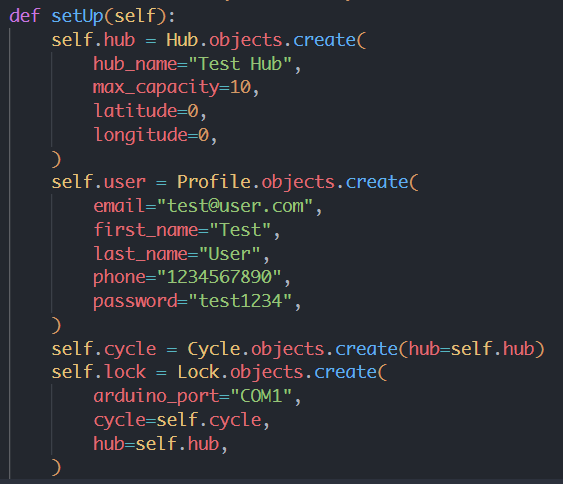
\includegraphics[scale=0.6]{unit_testing_codes/start_ride_setup.png}
\end{center}
The edge cases are tested as follows
\begin{center}
    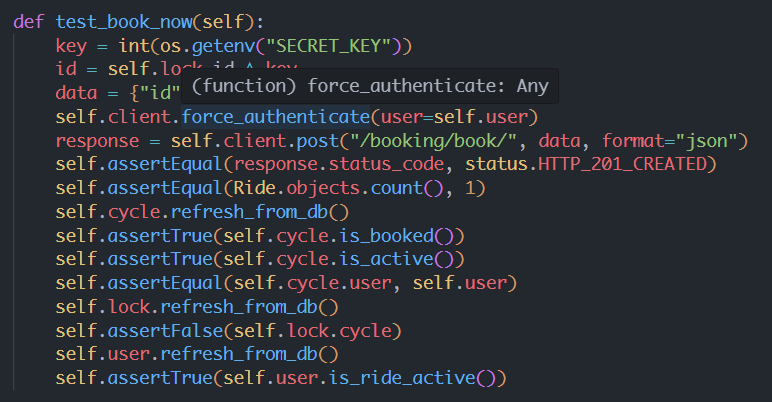
\includegraphics[scale=0.5]{unit_testing_codes/start_ride_1.png}\\
    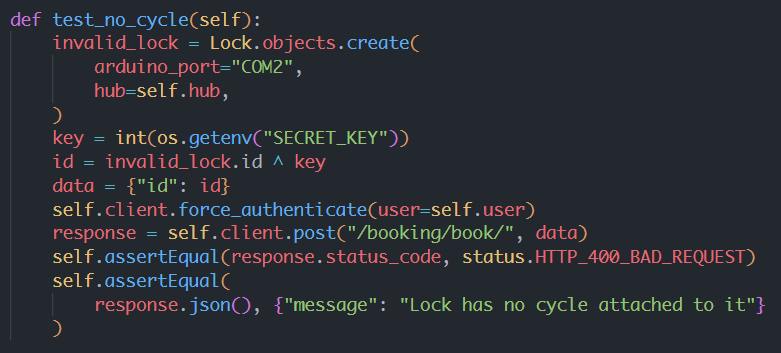
\includegraphics[scale=0.7]{unit_testing_codes/start_ride_2.png}\\
    Lock has no cycle attached to it\\
    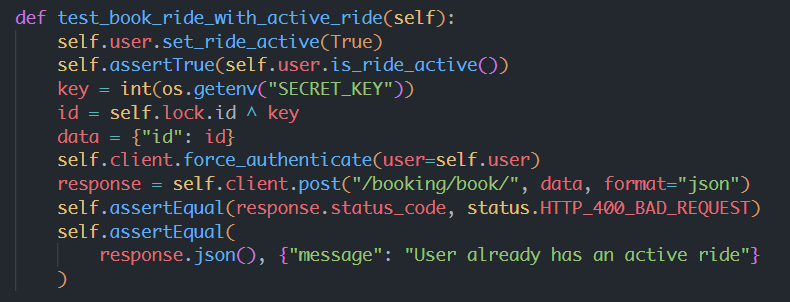
\includegraphics[scale=0.7]{unit_testing_codes/start_ride_3.png}\\
    User already has an active ride\\
    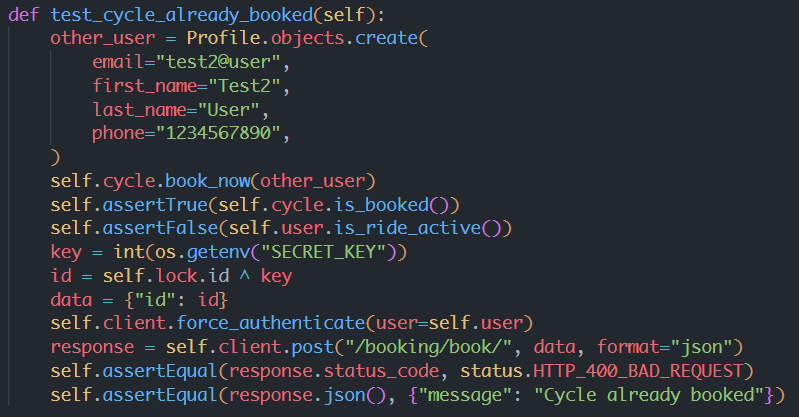
\includegraphics[scale=0.7]{unit_testing_codes/start_ride_4.png}\\
    Cycle is already booked by another user\\
    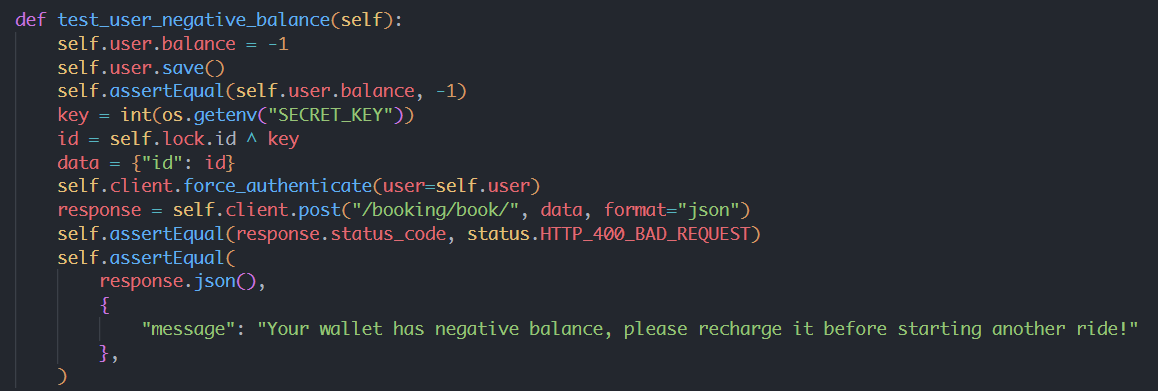
\includegraphics[scale=0.5]{unit_testing_codes/start_ride_5.png}
    User has negative balance in their wallet
\end{center}


\subsubsection{Ending Ride}
\textbf{API Endpoint: } \texttt{/booking/end/} \\
\textbf{Test Owner: } Khushi Gupta \\
\textbf{Date: } 26/03/2024 \\
\textbf{Test Description: } This test case is used to check if a user can end a ride successfully. \\
\textbf{Test Results: } User is able to end the ride successfully by scanning the QR code on the lock. The following edge cases were tested -
\begin{itemize}
    \itemsep 0em
    \item If the QR code is invalid, appropriate error message is shown.
    \item If the lock is already attached to another cycle, appropriate message is shown.
    \item If the user does not have an active ride, appropriate message is shown.
\end{itemize}

The test database is initialized as follows
\begin{center}
    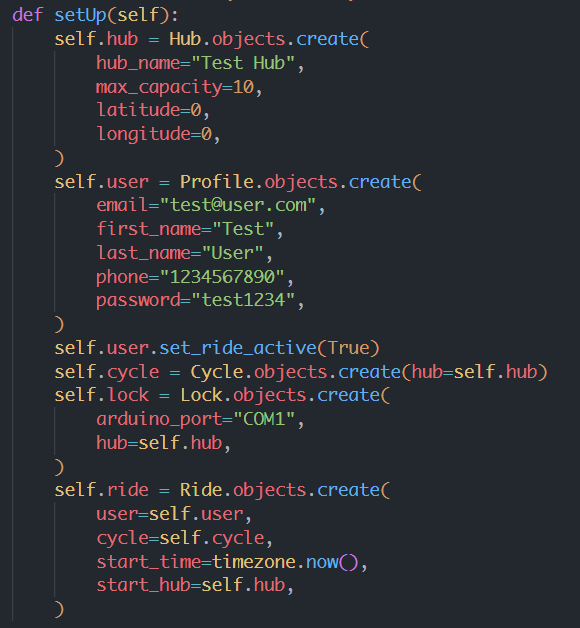
\includegraphics[scale=0.6]{unit_testing_codes/end_ride_setup.png}
\end{center}

The edge cases are tested as follows
\begin{center}
    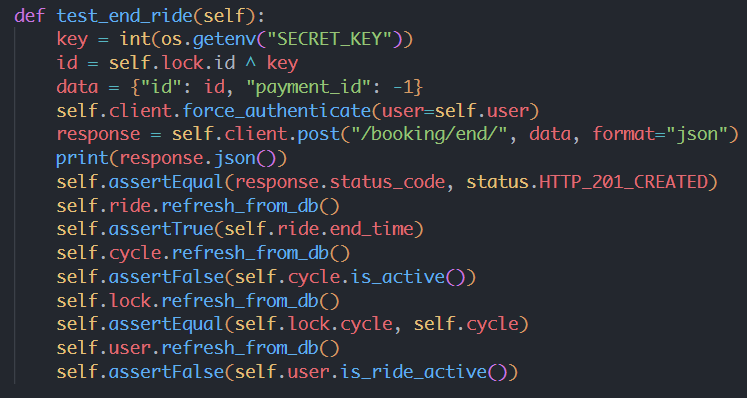
\includegraphics[scale=0.75]{unit_testing_codes/end_ride_1.png}\\
    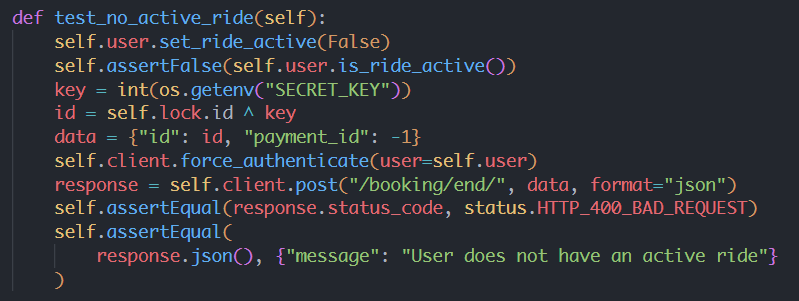
\includegraphics[scale=0.7]{unit_testing_codes/end_ride_2.png}\\
    User does not have an active ride\\
    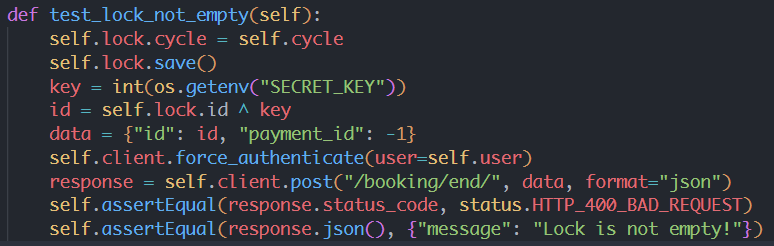
\includegraphics[scale=0.72]{unit_testing_codes/end_ride_3.png}\\
    Lock is already attached to another cycle\\
\end{center}

\subsubsection{Booking a Cycle for Later}
\textbf{API Endpoint: } \texttt{/booking/book\_later/} \\
\textbf{Test Owner: } Nevish Pathe \\
\textbf{Date: } 26/03/2024 \\
\textbf{Test Description: } This test case is used to check if a subscribed user can book a cycle for later. \\
\textbf{Test Results: } User is able to book a cycle for later successfully. The following edge cases were tested -
\begin{itemize}
    \itemsep 0em
    \item If the user has insuffienct balance in their wallet, they are denied to book a cycle.
    \item If the user has not subscribed to the service, they are denied to book a cycle for later.
    \item If the desired cycle is already booked by some other user, appropriate message is shown.
    \item If the desired start time is in the past, appropriate message is shown.
    \item If there is no cycle available at the desired hub, appropriate message is shown.
\end{itemize}

The test database is initialized as follows
\begin{center}
    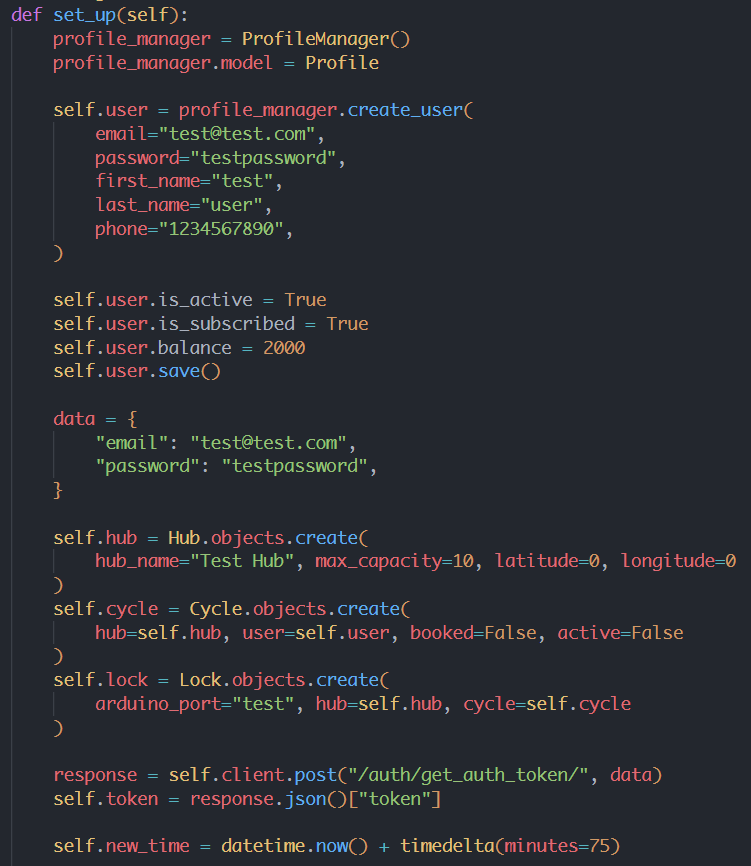
\includegraphics[scale=0.75]{unit_testing_codes/book_later_setup.png}
\end{center}

The edge cases are tested as follows

\begin{center}
    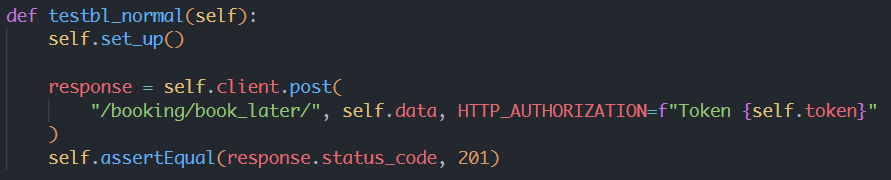
\includegraphics[scale=0.7]{unit_testing_codes/book_later_1.png}\\
    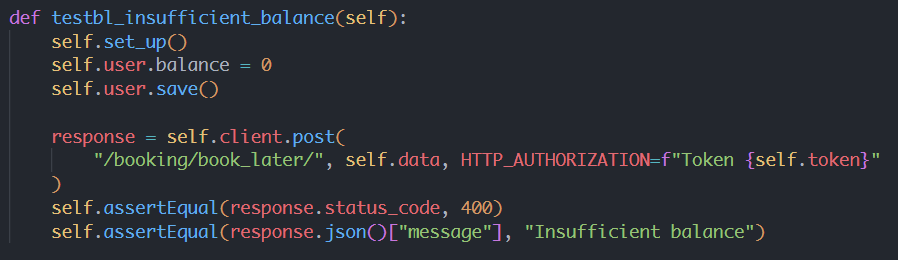
\includegraphics[scale=0.7]{unit_testing_codes/book_later_2.png}\\
    User has insufficient balance in their wallet\\
    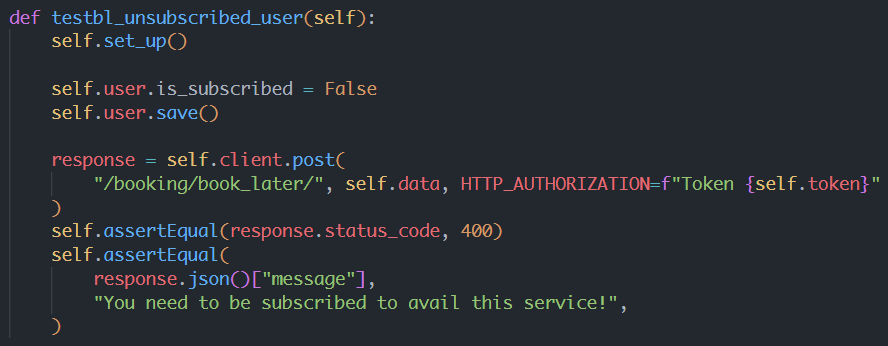
\includegraphics[scale=0.7]{unit_testing_codes/book_later_3.png}\\
    User has not subscribed to the service\\
    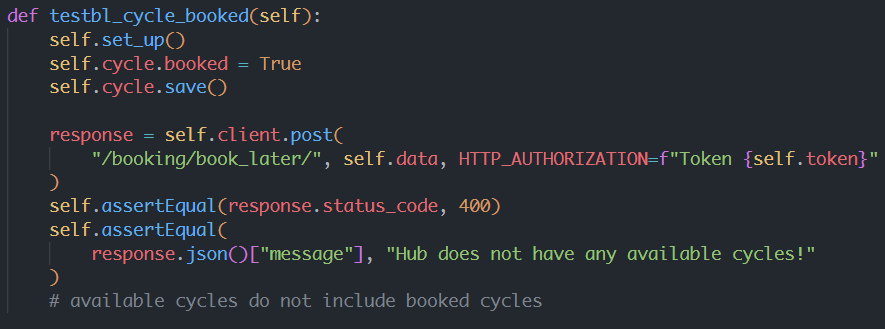
\includegraphics[scale=0.7]{unit_testing_codes/book_later_4.png}\\
    Cycle is already booked by another user\\
    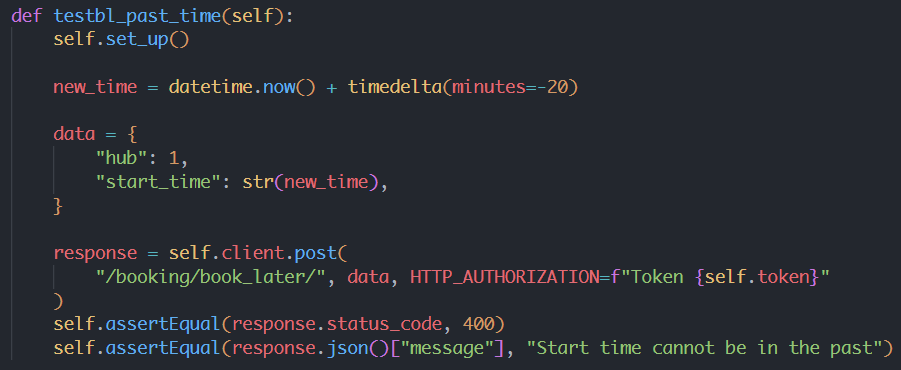
\includegraphics[scale=0.6]{unit_testing_codes/book_later_5.png}\\
    Desired start time is in the past\\
    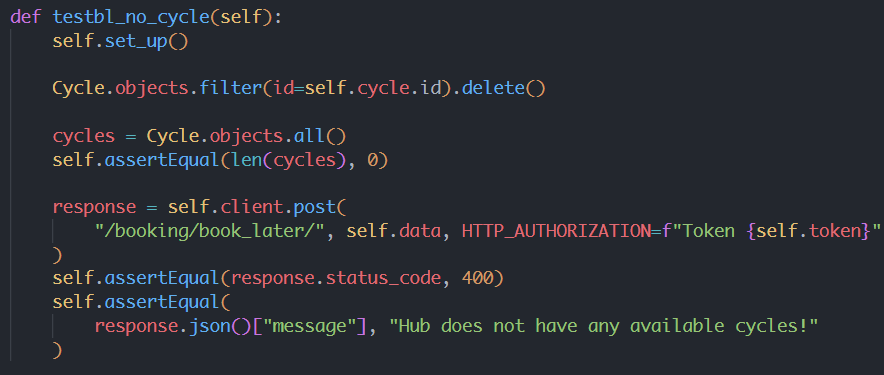
\includegraphics[scale=0.6]{unit_testing_codes/book_later_6.png}\\
    No cycle available at the desired hub\\
\end{center}

\subsubsection{Getting Details of Each Hub}
\textbf{API Endpoint: } \texttt{/booking/view\_hubs/} \\
\textbf{Test Owner: } Nevish Pathe \\
\textbf{Date: } 26/03/2024 \\
\textbf{Test Description: } This test case is used to check if a user can get the details of each hub. \\
\textbf{Test Results: } User is able to get the details of each hub successfully.\\
The database is pre-populated with various hub details in the \texttt{setUp()} method.

\begin{center}
    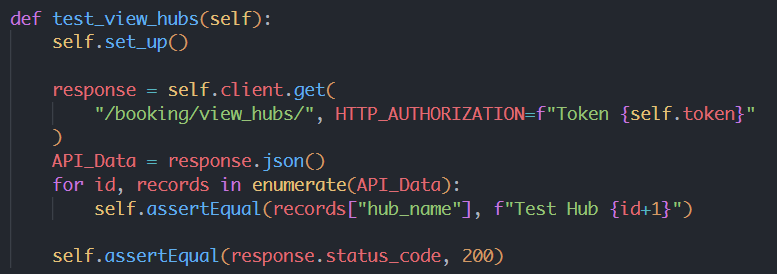
\includegraphics[scale=0.7]{unit_testing_codes/view_hubs.png}
\end{center}

\subsection{User Analytics}
\subsubsection{Viewing Ride History}
\textbf{API Endpoint: } \texttt{/analytics/history/} \\
\textbf{Test Owner: } Kaneez Fatima \\
\textbf{Date: } 25/03/2024 \\
\textbf{Test Description: } This test case is used to check if a user can view their ride history. \\
\textbf{Test Results: } User is able to view their ride history successfully.\\
The database is initialized with multiple rides in the \texttt{setUp()} method.
\begin{center}
    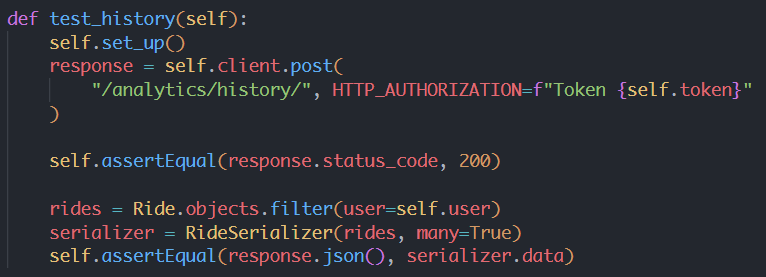
\includegraphics[scale=0.8]{unit_testing_codes/ride_history.png}
\end{center}

\subsubsection{Viewing Past Bookings}
\textbf{API Endpoint: } \texttt{/analytics/booking\_history/} \\
\textbf{Test Owner: } Kaneez Fatima \\
\textbf{Date: } 25/03/2024 \\
\textbf{Test Description: } This test case is used to check if a user can view their past and active bookings. \\
\textbf{Test Results: } User is able to view their past bookings successfully.\\
The database is initialized with multiple bookings in the \texttt{setUp()} method.
\begin{center}
    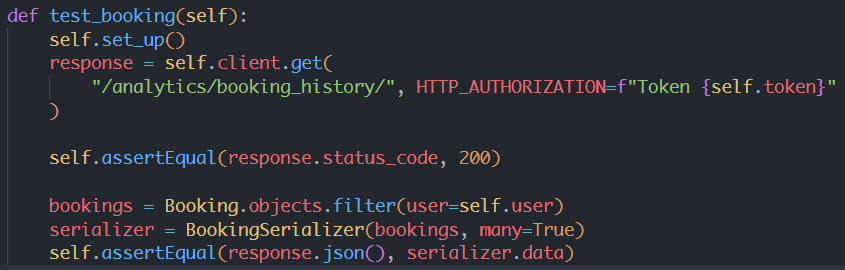
\includegraphics[scale=0.7]{unit_testing_codes/booking_history.png}
\end{center}

\subsection{Maintenance}
\subsubsection{Reporting an Issue}
\textbf{API Endpoint: } \texttt{/maintenance/feedbacks/add/} \\
\textbf{Test Owner: } Ananya Baghel \\
\textbf{Date: } 28/03/2024 \\
\textbf{Test Description: } This test case is used to check if a user can report an issue with the cycle. \\
\textbf{Test Results: } User is able to report an issue with the cycle successfully.\\

\begin{center}
    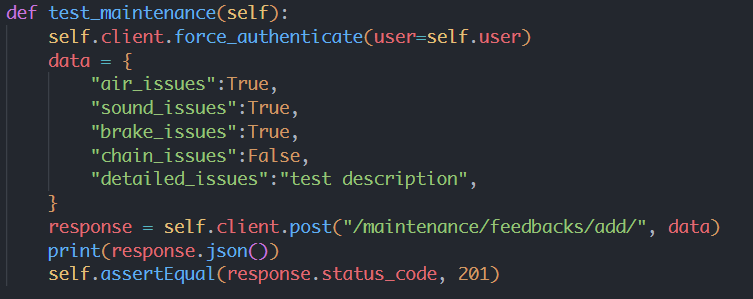
\includegraphics[scale=0.7]{unit_testing_codes/report_issue.png}
\end{center}

\subsection{Payment}
\subsubsection{Getting Wallet Balance}
\textbf{API Endpoint: } \texttt{/payment/get\_balance/} \\
\textbf{Test Owner: } Ananya Baghel \\
\textbf{Date: } 28/03/2024 \\
\textbf{Test Description: } This test case is used to check if a user can get their wallet balance. \\
\textbf{Test Results: } User is able to get their wallet balance successfully.\\

\begin{center}
    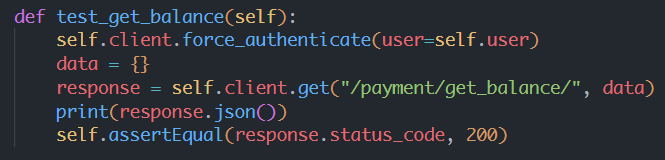
\includegraphics[scale=0.7]{unit_testing_codes/get_balance.png}
\end{center}

\subsubsection{Updating Wallet Balance}
\textbf{API Endpoint: } \texttt{/payment/update\_balance/} \\
\textbf{Test Owner: } Ananya Baghel \\
\textbf{Date: } 28/03/2024 \\
\textbf{Test Description: } This test case is used to check if a user can update their wallet balance. \\
\textbf{Test Results: } User is able to update their wallet balance successfully.\\

\begin{center}
    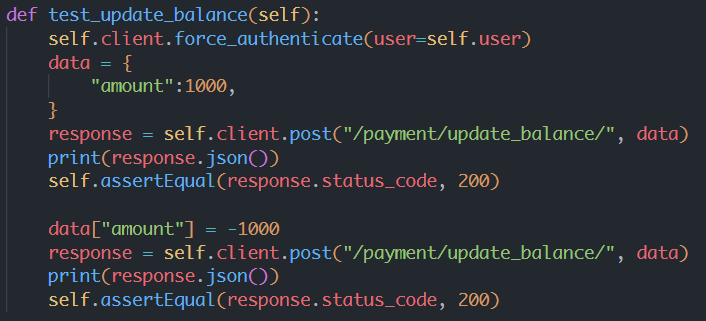
\includegraphics[scale=0.7]{unit_testing_codes/update_balance.png}
\end{center}

\subsubsection{Viewing Transaction History}
\textbf{API Endpoint: } \texttt{/payment/get\_transactions/} \\
\textbf{Test Owner: } Ananya Baghel \\
\textbf{Date: } 28/03/2024 \\
\textbf{Test Description: } This test case is used to check if a user can view their transaction history. \\
\textbf{Test Results: } User is able to view their transaction history successfully.\\

\begin{center}
    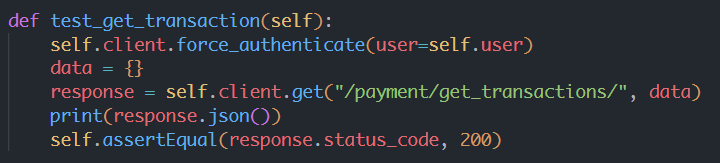
\includegraphics[scale=0.8]{unit_testing_codes/transaction_history.png}
\end{center}

\newpage
\section{\centering{\textbf{Integration Testing}}}

\subsection{Authentication}

\subsubsection{Registering a User}
\textbf{Module Details: }This module integrates the registration process for new users, providing the necessary functionality to create an account.
\\
\textbf{Test Owner: }Srishti Chandra
\\
\textbf{Test Date: }27/03/2024
\\
\textbf{Test Results: }
\begin{itemize}
    \item \textbf{Test Case 1: }Invalid name, phone number, or email address is entered.
    \\
    \textbf{Result: }Error messages are displayed in red text below the respective entry fields:
    \\
    - "Please enter your full name" is displayed if the full name field is left blank or contains only whitespace characters.
    \\
    - "Enter a valid phone number" is displayed if an invalid phone number format is entered.
    \\
    - "Enter a valid email address" is displayed if an invalid email address format is entered.

    \item \textbf{Test Case 2: }Valid name, phone number, and already registered email address are entered in the respective fields.
    \\
    \textbf{Result: }An alert dialog is triggered, notifying the user of an existing profile associated with the provided email address.

    \item \textbf{Test Case 3: }Valid name, phone number, and unregistered email address are entered in the respective fields.
    \\
    \textbf{Result: }Upon successful registration, the user is directed to the Account Created page. Here, instructions are given to activate the account via an email link. Clicking "Continue" on this page leads the user to the login page.

\end{itemize}
\textbf{Additional Comments: }Any trailing whitespace in the Full Name field should be removed and the full name must contain first and last name to ensure that the textbox recognizes the entry as complete.


\subsubsection{Logging in a User}
\textbf{Module Details: }This module is integration of all the components of the login page.
\\
\textbf{Test Owner: }Srishti Chandra
\\
\textbf{Test Date: }27/03/2024
\\
\textbf{Test Results: }
\begin{itemize}
    \item \textbf{Test Case 1: }If the user has not signed up and attempts to log in with an unregistered email ID and password.
    \\
    \textbf{Result: }An alert prompt is displayed that conveys that no such user exists.

    \item \textbf{Test Case 2: }If the user has not signed up and attempts to sign up.
    \\
    \textbf{Result: }The user can click on the "Not on Pedal Pal Yet? Sign Up!" link located at the bottom of the screen, which redirects them to the registration page.

    \item \textbf{Test Case 3: }Invalid email ID is entered, such as incorrect formatting or other issues.
    \\
    \textbf{Result: }An error message in red text is displayed below the email input field, indicating "Invalid email address format."

    \item \textbf{Test Case 4: }Incorrect password is entered with a registered email ID.
    \\
    \textbf{Result: }An alert prompt is displayed that conveys “Incorrect  Password”.

    \item \textbf{Test Case 5: }User doesn’t remember the password.
    \\
    \textbf{Result: }Clicking on "Forgot Password" redirects to the Forgot Password page.

    \item \textbf{Test Case 6: }Registered email ID and password are entered, and the Login button is clicked.
    \\
    \textbf{Result: }The user is successfully redirected to the Homepage of Pedalpal.

\end{itemize}
\textbf{Additional Comments: }None

\subsubsection{Email Verification}

\subsubsection{Forgot Password}

















\subsection{Wallet: Transaction History and Add Balance}
\textbf{Module Details: }This module includes tests for:
\begin{itemize}
    \item Transaction Logs of the in-app Wallet, featuring payments made while using app.
    \item Functionality of adding balance to the wallet.
\end{itemize}
\textbf{Test Owner: }Raghav Manglik
\\
\textbf{Test Date: }[ 26-03-2024 - 27-03-2024 ]
\\
\textbf{Test Results: }


\begin{itemize}
    \item \textbf{Test case 1: }An unsubscribed user attempts to access the wallet, which is a service that requires a subscription.
    \\
    \textbf{Result: }An alert prompt is displayed telling user that this feature is available only for subscribed users.
    \item \textbf{Test case 2: }After subscribing, A user tries to access the wallet.
    \\
    \textbf{Result: }My Wallet page is displayed, showing the current balance after deducting subscription fee of Rs.20  from predetermined amount of Rs.100 along with option to Add balance and View Transaction History
    \item \textbf{Test case 3: }A user tries to view Transaction History.
    \\
    \textbf{Result: }Transaction history page displaying credit and debit of balance with green and red colour respectively are shown.
    \item \textbf{Test case 4: }A user tries to add Rs.0 to wallet.
    \\
    \textbf{Result: }The Razorpay payment gateway fails to operate correctly without displaying any error messages. ( DEBUG NEEDED )
    \item \textbf{Test case 5: }A user tries to copy/cut and paste an invalid amount (-ve amount or a string of characters) in Add Balance window.
    \\
    \textbf{Result: }Only leading numerical values are pasted in the Enter Amount box. 
    \item \textbf{Test case 6: }A user tries to enter more than 2 digits after the decimal point / any symbol other than a single decimal point in Enter Amount Box in Add Balance window.
    \\
    \textbf{Result: }The input restricts user to enter no more than two digits after the decimal point, while also restricting the entry of invalid symbols and permitting only a single decimal point.






    
    
\end{itemize}



\textbf{Additional Comments: } [WHAT TO BE CHANGED AFTER DEBUG]




\subsection{Ride History Page}
\textbf{Module Details: }This module includes tests for viewing bicycle renting logs.
\\
\textbf{Test Owner: }Raghav Manglik
\\
\textbf{Test Date: }[ 26-03-2024 - 27-03-2024 ]
\\
\textbf{Test Results: }
\begin{itemize}
    \item \textbf{Test Case 1: }A user who hasn't rented bicycles before accesses the History page.
    \\
    \textbf{Result: }History Page is displayed with Total time used 0h 0m and no record of any ride.
    \item \textbf{Test Case 2: }A user while riding, that is with an active ride, accesses the History Page.
    \\
    \textbf{Result: }The History Page is displayed with information regarding past rides and no details about the active ride.
\end{itemize}
\textbf{Additional Comments: }The discrepancy between the starting and ending times compared to the duration shown in the middle below the arrow arises from the system factoring in seconds in its calculation.

\subsection{My Booking Page}
\textbf{Module Details: }This module includes tests for accessing logs for both past bicycle bookings and currently active bookings.
\\
\textbf{Test Owner: }Raghav Manglik
\\
\textbf{Test Date: }[ 26-03-2024 - 27-03-2024 ]
\\
\textbf{Test Results: }
\begin{itemize}
    \item \textbf{Test Case 1: }An unsubscribed user accesses My Bookings page, a subscription required service.
    \\
    \textbf{Result: }My Bookings Page is displayed with both Current and Past Bookings as 0.
    \item \textbf{Test Case 2: }A user who hasn't booked any bicycle before accesses My Bookings page.
    \\
    \textbf{Result: }My Bookings Page is displayed with both Current and Past Bookings as 0.
    \item \textbf{Test Case 3: }A Bicycle is booked for a finite time and My Bookings Page is accessed.
    \\
    \textbf{Result: }My bookings page is displayed with current bookings incremented and showing the details about the booking. Initially, The bicycle remained in Current Bookings section once the booking period expired. This was subsequentially rectified as once the booking period expired, The bicycle moved to Past Bookings section.

\end{itemize}
\textbf{Additional Comments: }The discrepancy between the starting and ending times of the booking compared to the duration shown arises from the system factoring in seconds in its calculation.

\subsection{View Profile Page and Subscribe}
\textbf{Module Details: }This module includes tests for accessing information about a user.
\\
\textbf{Test Owner: }Raghav Manglik
\\
\textbf{Test Date: }[ 26-03-2024 - 27-03-2024 ]
\\
\textbf{Test Results: }
\begin{itemize}
    \item \textbf{Test Case 1: }A user navigates to their Profile Page.
    \\
    \textbf{Result: }Profile Page is displayed with their Name, Email, Phone, Subscription Status and a default Profile picture. If the user is not subscribed, an additional button is displayed on their Profile Page to navigate to the subscription option. Clicking this button opens the Razorpay payment gateway, which charges Rs.100. Out of this amount, Rs.80 is added to the user's wallet, and Rs.20 is deducted as the subscription fee.
    \item \textbf{Test Case 2: }A user attempts to change their profile picture by clicking on a camera icon beside the profile picture.
    \\
    \textbf{Result: }The feature to change Personal Information along with Profile Picture is yet to be implemented. Currently clicking on that icon does nothing.
\end{itemize}
\textbf{Additional Comments: }

\newpage
\section{\centering{\textbf{System Testing}}}
\subsection{Functional Requirements}
\subsection{Non-Functional Requirements}
\subsubsection{Performance Requirements}
\textbf{Test Owner: }Amogh Bhagwat\\
\textbf{Date: }30/03/2024\\
\textbf{Test Description: }This test case is used to check the response time of the backend server.\\
\textbf{Test Results: }The response time of the backend server APIs is less than 1 second.\\

\begin{center}
    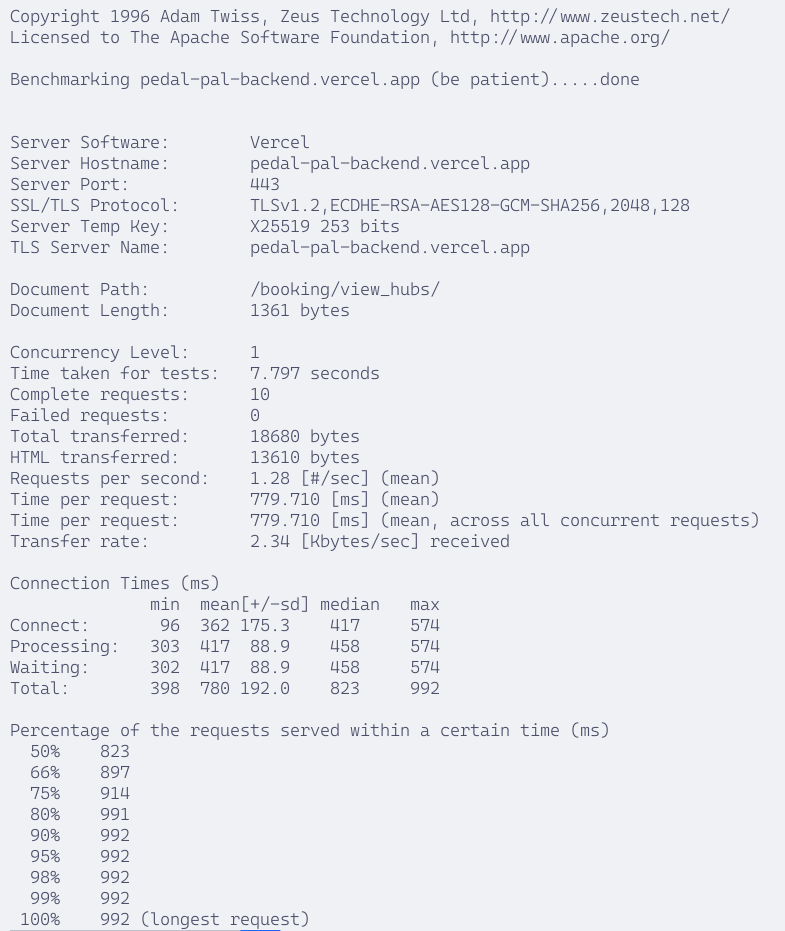
\includegraphics[scale=0.6]{unit_testing_codes/load_testing.png}
\end{center}
\textbf{Additional Comments: }The response time of the backend server APIs is less than 1 second only when the server is already active. Since we are using Vercel's free plan,  the server goes to sleep after 5 minutes of inactivity. The first request after the server wakes up takes around 10-30 seconds.

\subsubsection{Security Requirements}
\begin{itemize}
    \itemsep 0em
    \item All user passwords are encrypted before storing them in the database. The user's password is never stored in plain text.
    \item All payments are done through Razorpay's secure payment gateway.
    \item All API calls between frontend and backend are authenticated using JWT tokens, and are encrypted using HTTPS.
\end{itemize}

\newpage
\section{\centering{\textbf{Conclusion}}}

\appendixpageoff
\begin{appendices}

\newpage

\section{\centering{\textbf{Group Log}}}
\begin{tabular}{|p{1cm}|p{2cm}|p{2cm}|p{2cm}|p{6.75cm}|}
\hline
\makecell{\textbf{S.No}} & \makecell{\textbf{Date}} & \makecell{\textbf{Timings}} & \makecell{\textbf{Venue}} & \makecell{\textbf{Description}} \\
\hline
\makecell{1} & \makecell{07/01/2024} & \makecell{14:00\\ to \\16:00} & \makecell{RM \\Building} & \makecell{Brain-stormed various possible \\ prospective ideas for the project. \\ Main ideas presented were: \\ Bicycle Rental Services \\ Hall Management \\ Used goods Buy/Sell Portal} \\
\hline
\makecell{2} & \makecell{09/01/2024} & \makecell{14:30\\to\\17:00} & \makecell{Google\\ Meet} & \makecell{Finalized the idea for the project and \\ discussed various aspects of it.} \\
\hline
\makecell{3} & \makecell{11/01/2024} & \makecell{22:00\\to\\00:00} & \makecell{Google\\Meet} & \makecell{Studied the SRS template given and \\ distributed the work amongst the team \\ members.} \\
\hline
\makecell{4} & \makecell{17/01/2024} & \makecell{21:00\\to\\21:30} & \makecell{Google\\Meet} & \makecell{First meet with the Teaching Assistant \\ Mr. Bharat. Discussed about project \\ and the SRS documentation.} \\
\hline
\makecell{5} & \makecell{20/01/2024} & \makecell{15:00\\to\\18:00} & \makecell{Google\\Meet} & \makecell{Brainstorming of final ideas and \\ discussion on use cases, features, \\ data flows.} \\
\hline
\makecell{6} & \makecell{21/01/2024} & \makecell{14:00\\to\\15:00} & \makecell{Google\\Meet} & \makecell{Decided to use Django with bootstrap \\ and inline CSS to build the front end \\ part of our application and PostgreSQL \\ as our DBMS.} \\
\hline
\makecell{7} & \makecell{22/01/2024} & \makecell{23:00\\to\\00:00} & \makecell{Google\\Meet} & \makecell{Explored more functionalities for the \\ product and progressed with the SRS \\ document.} \\
\hline
\makecell{8} & \makecell{25/01/2024} & \makecell{14:00\\to\\17:00} & \makecell{RM\\Building} & \makecell{Finalized the SRS Document and\\completed typesetting in \LaTeX} \\
\hline
\end{tabular}
\end{appendices}
\end{document}
